\documentclass{article}
\usepackage[utf8]{inputenc}
\usepackage[UTF8]{ctex}
\usepackage{amsthm}
\usepackage{amsmath}
\usepackage{amssymb}
\usepackage{graphicx}
\usepackage{hyperref}
\usepackage[table]{xcolor}
\usepackage{fancyhdr}
\usepackage{lastpage}
\usepackage{pythonhighlight}
\usepackage{subfigure}
\usepackage{fancyhdr}
\usepackage[superscript]{cite}
\usepackage{geometry}

\geometry{left=3cm,right=3cm,top=1.5cm,bottom=1.5cm}
\begin{document}
\title{木星磁场的建模与计算}
\author{薛昊天 518021910506}
\date{}

\maketitle
\begin{abstract}
   木星作为太阳系最大的行星,拥有最强的行星磁场。木星磁场是木星探测的基本环境之一,因此对木星磁场的建模很有意义。本文通过借鉴国际地磁场的建模计算过程,在木星上类比计算出磁场强度。\\
  \textbf{关键词:木星,磁场,建模}
  
\end{abstract}




\section{建模过程}
 \subsection{基本假设}
   在本文中,我们假设木星是一个规则球体,半径为$R_J$,参考系使用 Right-handed System III
   (S3RH), 如图1:在这一参考系下,木星表面一个点的经度$\lambda_{RH}$随着自传而减小。
   同时我们假设木星内部的磁场是由恒定电场产生的稳恒磁场,是一个有势无旋场。
   
\begin{figure}
    \centering
    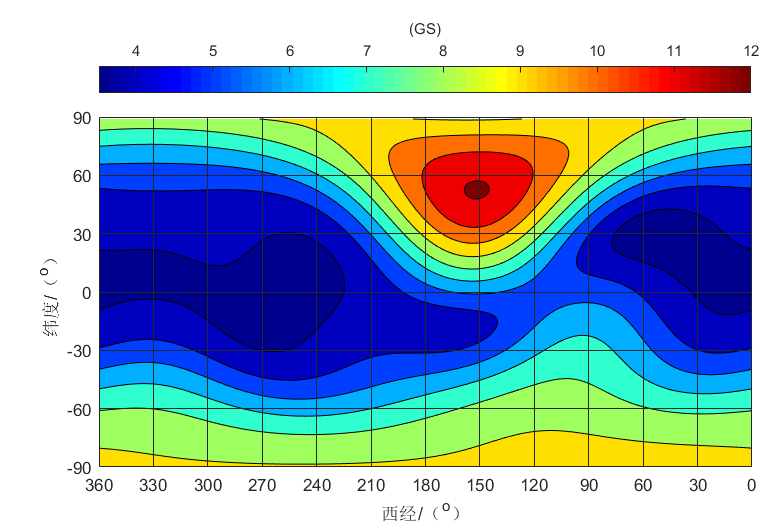
\includegraphics[scale=0.3]{./figure/model.pdf}
    \caption{S3RH木星坐标系}
    \label{fig:my_label}
\end{figure}   

   \subsection{公式}
   首先在麦克斯韦方程组中,在稳恒场中有:
   
   \begin{equation} 
       \nabla \times E = \frac{\partial{B}}{\partial{t}} 
   \end{equation}

   而根据假设的电场条件,有 $E=-\nabla{\varphi}$。在S3RH参考系下,有$\varphi=U(r,\theta,\lambda)$,代入式(1)有:
   
   \begin{equation} 
       \nabla^{2}\varphi=\nabla^{2}U(r,\theta,\lambda)=0
   \end{equation}
   这是一个球坐标下的拉普拉斯方程,表达式可以求出是:

    \begin{equation}
        \frac{1}{r^{2}}\frac{\partial}{\partial{r}}(r^2\frac{\partial{U}}{\partial{r}})+\frac{1}{r^2sin\theta}\frac{\partial}{\partial\theta}(sin\theta\frac{\partial{U}}{\partial\theta}) + \frac{1}{r^2sin^2\theta}\frac{\partial^{2}U}{\partial{\lambda}^2}=0
   \end{equation}
   
分离变量r,有:
     \begin{equation} 
      U(r,\theta,\lambda) = R(r)Y(\theta, \lambda)
   \end{equation}
   
代入(3)变形可以得到:
\begin{equation} 
      \frac{1}{R}\frac{d}{dr}(r^2\frac{dR}{dr}) = \frac{1}{sin\theta{Y}}\frac{\partial}{\partial\theta}(sin\theta\frac{\partial{Y}}{\partial{\theta}})-\frac{1}{Y}\frac{1}{r^2sin\theta}\frac{\partial^2Y}{\partial\lambda^2}   
   \end{equation}
   
 上面等式的左边是关于r的函数,右边是关于$\theta,\lambda$的函数,所以由自变量的任意性可以知道等式两边都恒等与某一个常数,记为$l(l+1)$,则可以将上述方程拆分成两个方程:
 \begin{equation}
         \frac{d}{dr}(r^2\frac{dR}{dr})-l(l+1)R=0      
 \end{equation}
 
 \begin{equation}
        \frac{1}{sin\theta}\frac{\partial}{\partianl\theta}(sin\theta\frac{\partial{Y}}{\partial\theta})+\frac{1}{sin^2\theta}\frac{\partial^2Y}{\partial\lambda^2}+l(l+1)Y=0
 \end{equation}
 其中方程(6)是一个欧拉型常微分方程,它的解是:
  \begin{equation}
      R(r)=Cr^{l} + Dr^{-l-1}
  \end{equation}
  方程(7)仍然是球函数方程,可以进一步分离变量:$Y(\theta,\lambda)=\Gamma(\theta)\Phi(\lambda)$
 代入(7)中,将$\theta$和$\lambda$有关的式子分别移到等式两侧得到:
 \begin{equation}
     \frac{sin\theta}{\Gamma}\frac{d}{d\theta}(sin\theta\frac{d\Gamma}{d\theta})+l(l+1)sin^2\theta=-\frac{1}{\Phi}\frac{d^2\Phi}{d\lambda^2}
 \end{equation}
 同样可以知道左右一定恒等与某一个常数,记做$\gamma$,代入(9)同样可以得到两个方程:
\begin{equation}
    \Phi^{''} + \gamma\Phi = 0
\end{equation}

\begin{equation}
    sin\theta\frac{d}{d\theta}(sin\theta\frac{\partial{\Gamma}}{\partial\theta})+(l(l+1)sin^2\theta-\gamma)\Gamma=0
\end{equation}
常微分方程(10)是容易解的,它的本征函为:
\begin{equation}
    \Gamma(\lambda)=Acosm\lambda+Bsinm\lambda
\end{equation}
再看方程(11),利用$arccosx=\theta$,用x作为唯一的自变量得:
\begin{equation}
    (1-x^2)\frac{d^2\Phi}{dx^2} - 2x\frac{d\Phi}{dx}+l(l+1)\Phi=0
\end{equation}
这是一个一阶连带勒让德方程。

所以综合上面的过程,我们就可以求解出木星表面磁场的表达式:
\begin{equation}
    U_i(r, \theta,\lambda)=R\sum_{n=1}^{\infty}\sum_{m=0}^{n}(\frac{R}{r})^{n+1}\times(g_{n}^{m}cos(m\lambda)+h_{n}^{m}sin(m\lambda))P^{m}_{n}(cos\theta)
\end{equation}
其中r是待测点的径向距离;$\theta$是S3RH中的余纬度,$\lambda$是东经度;$g_n^m,h_n^m$是球谐系数,$P_n^m(x)$是n阶m次的施密特半标准化缔合勒让德函数。更具$\textbf{B}=-\nabla\textbf{U}$可得磁场在三个方向上的分量:

%\includegraphics[scale=1.2]{./figure/ans.PNG}

\begin{equation}
  \left\{
    \begin{array}{l}\vspace{1ex} 
            B_{\theta}=-\frac{\partial{U}}{r\partial\theta}= -R\sum_{n=1}^{\infty}\sum_{m=0}^{n}(\frac{R}{r})^{n+1}\times(g_{n}^{m}cos(m\lambda)+h_{n}^{m}sin(m\lambda))\frac{P^{m}_{n}(cos\theta)}{\partial\theta}\\ \vspace{1ex} 
            B_{\lambda}=-\frac{\partial\varphi_i}{rsin\theta\partial\lambda}=R\sum_{n=1}^{\infty}\sum_{m=0}^{n}(\frac{R}{r})^{n+1}\times(g_{n}^{m}cos(m\lambda)-h_{n}^{m}sin(m\lambda))P^{m}_{n}(cos\theta) \\ \vspace{1ex} 
            B_r = -\frac{\partial\varphi_i}{\partial{r}}=R\sum_{n=1}^{\infty}\sum_{m=0}^{n}(n+1)(\frac{R}{r})^{n+1}\times(g_{n}^{m}cos(m\lambda)+h_{n}^{m}sin(m\lambda))P^{m}_{n}(cos\theta)
            
        \end{array}
\right.
\end{equation}


公式(15)也是我们计算的主要依据,需要注意的是公式里面的$g_n^m,h_n^m$到目前为止还是未知的,我们可以通过测量得到的一些边界值来解出这些球谐系数。





\section{计算过程}


\subsection{计算准备}
  我们在这里使用MATLAB进行计算,计算公(15)式里面施密特半标准化缔合勒让德函数是MATLAB内置的。表达式里的球谐系数使用VIT4模型提出的球谐系数,见表(1):

\begin{figure}
    \centering
    \includegraphics[scale=0.4]{./TABLE.PNG}  
    \caption{VIT4模型中的球谐系数}
    \label{fig:my_label}
\end{figure}



\subsection{计算流程}


\subsection{计算结果}



\begin{figure}
    \centering
    \includegraphics[scale=0.25]{./figure/demo.jpg}
    \caption{利用Matlab模拟出的木星磁场的分布情况}
    \label{fig:my_label}
\end{figure}



\section{总结}



\section{致谢}



\end{document}
